% --------------------------------------------------------------
% This is all preamble stuff that you don't have to worry about.
% Head down to where it says "Start here"
% --------------------------------------------------------------

\documentclass[12pt]{article}
\usepackage[margin=0.75in]{geometry}
\usepackage{amsmath,amsthm,amssymb,mathtools,graphicx,enumitem,hyperref,hyphenat,float}
% \usepackage[paperwidth=\maxdimen,paperheight=\maxdimen]{geometry}
\usepackage{svg}
\usepackage{register}
\usepackage{rotating}
\DeclarePairedDelimiter{\ceil}{\lceil}{\rceil}
\newcommand{\N}{\mathbb{N}}
\newcommand{\Z}{\mathbb{Z}}
\newcommand{\Q}{\mathbb{Q}}
\newcommand{\R}{\mathbb{R}}
\newcommand{\F}{\mathbb{F}}
\newcommand{\C}{\mathbb{C}}
\newcommand{\lub}{\mathrm{lub}}
\newcommand{\g}{\mathrm{glb}}
\newcommand{\seq}{\subseteq}
\newcommand{\e}{\epsilon} 
\newcommand{\de}{\delta}
\newcommand{\mbf}{\mathbf}
\newcommand{\es}{\emptyset}
\newcommand{\mc}{\mathcal}
\newcommand{\un}{\cup}
\newcommand{\ic}{\cap}
\newcommand{\gen}[1]{\ensuremath{\langle #1\rangle}}
\newcommand{\spn}{\mathrm{span \ }}
\newcommand{\dm}{\mathrm{dim \ }}
\newcommand{\Lm}{\mathcal{L}}
\newcommand{\nll}{\mathrm{null \ }}
\newcommand{\rng}{\mathrm{range \ }}
\newcommand{\dgr}{\mathrm{deg \ }}
\newcommand{\Lim}{\lim\limits}
\newcommand{\Sum}{\sum\limits}
\newcommand{\Pt}{\|P\|}
\newcommand{\dmn}{\mathrm{dom \ }}
\newcommand{\Prod}{\prod\limits}
\DeclarePairedDelimiter\floor{\lfloor}{\rfloor}
\DeclarePairedDelimiter\ev{\langle}{\rangle}
\newcommand*\dif{\mathop{}\!\mathrm{d}}
\newcommand{\Beta}{\mathcal B}
\newcommand{\Seq}{\mathrm{Seq }}
\theoremstyle{plain}

\newtheorem{thm}{Theorem} % reset theorem numbering for each chapter
\newtheorem{lem}{Lemma}
\newtheorem{cor}{Corollary}
\newtheorem{rem}{Remark}
\newtheorem{fct}{Fact}
\newtheorem{cnj}{Conjecture}
\newtheorem{asm}{Assumption}
\theoremstyle{definition}
\newtheorem{defn}{Definition}
\newtheorem{exmp}{Example} % same for example numbers
\renewcommand{\regBitWidth}{16}
	
\begin{document}
	
% --------------------------------------------------------------
%                         Start here
% --------------------------------------------------------------
	
\begin{titlepage}

	\newcommand{\HRule}{\rule{\linewidth}{0.5mm}} % Defines a new command for the horizontal lines, change thickness here
	
	\center % Center everything on the page
	 
	%----------------------------------------------------------------------------------------
	%	HEADING SECTIONS
	%----------------------------------------------------------------------------------------
	
	\textsc{\LARGE Faculty of Engineering, Cairo University}\\[0.5cm] % Name of your university/college
	\textsc{\large Computer Engineering Department}\\[1.5cm] % Minor heading such as course title
	
	\textsc{\Large Computer Architecture Course Project}\\[0.5cm] % Major heading such as course name
	
	%----------------------------------------------------------------------------------------
	%	TITLE SECTION
	%----------------------------------------------------------------------------------------
	
	\HRule \\[0.4cm]
	{ \huge \bfseries Orthrus - Phase 1 Report}\\[0.4cm] % Title of your doc
	\HRule \\[1.5cm]
	 
	%----------------------------------------------------------------------------------------
	%	AUTHOR SECTION
	%----------------------------------------------------------------------------------------
	
	\begin{minipage}{0.4\textwidth}
	\begin{flushleft} \large
	Ahmad Khaled \\
	Maryam Shalaby \\
	Zeinab Rabie \\
	Omnia Zakaria
	\end{flushleft}
	\end{minipage}
	\begin{minipage}{0.4\textwidth}
	\begin{flushright}\large
        Section 1 BN. 03 \\
        Section 2 BN. 21 \\
        Section 1 BN. 22 \\
        Section 1 BN. 23 \\
	\end{flushright}
	\end{minipage}\\[1cm]
	
	% If you don't want a supervisor, uncomment the two lines below and remove the section above
	%\Large \emph{Author:}\\
	%John \textsc{Smith}\\[3cm] % Your name
	
	%----------------------------------------------------------------------------------------
	%	LOGO SECTION
	%----------------------------------------------------------------------------------------
	
	
\includegraphics[scale=0.15]{cu_logo.png}\\[1cm] % Include a department/university logo - this will require the graphicx package
	 
	%----------------------------------------------------------------------------------------
	
	\vfill % Fill the rest of the page with whitespace
	
\end{titlepage}

\tableofcontents

\section{Introduction}
Orthrus is a pipelined static dual-issue microprocessor implementing a RISC ISA similar to the MIPS ISA. In the following sections we outline the instruction format, the general design of the processor, as well as the pipeline stages design.

\section{Instruction Set Architecture}
    The structure for the IR for One-Operand instructions is given in Figure~\ref{IR-1op}.The structure for the IR for Two-Operand instructions is given in Figure~\ref{IR-2op}. The structure for the IR for Memory instructions is given in Figure~\ref{IR-memory}. The structure for the IR for Branch & Change of Control instructions is given in Figure~\ref{IR-Branch}.
    \begin{table}[H]
        \centering
        \begin{tabular}{c|c|c|c|c|}
            \cline{2-5}
                            & $R_0$ & $R_1$ & $R_2$ & $R_3$ \\ \cline{2-5} 
            \textit{Code}   & 000      & 001            & 010            & 011     \\ \cline{2-5} 
                            & $R_4$ & $R_5$ & $R_6?$ & $R_7$ \\ \cline{2-5} 
            \textit{Code}   & 100      & 101            & 110            & 111     \\ \cline{2-5} 
        \end{tabular}
        \caption{Register Addressing Codes}
        \label{reg-addr-codes}
    \end{table}
    \begin{table}[H]
        \centering
        \begin{tabular}{|c|c|c|c|c|c|c|c|c|}
            \hline
            Instruction  & NOP & SETC & CLRC  & NOT & INC & DEC & OUT & IN  \\ \hline
            OP Code     & 00000 & 00001 & 00010 & 00011 & 00100 & 00101 & 00110 & 00111 \\ \hline
        \end{tabular}
        \caption{One-Operand Instruction Codes}
        \label{One_Op Opcodes}
    \end{table}
    
    \begin{figure}[H]
        \centering
        \caption{IR Structure For One-Operand Instructions}
        \label{IR-1op}
        \vspace{0.5 cm}
        \regfield{}{5}{11}{{Instruction}}
        \regfield{}{3}{8}{{Destination Register}}
        \regfield{}{8}{0}{{}}
        \\
        \vspace{0.5 cm}
        \begin{regdesc}\begin{reglist}
            \item [Instruction] specifies the instruction to execute. Possible codes given in. Table~\ref{One_Op Opcodes}.
            \item [Destination Register] specifies the destination register. Possible codes given in Table~\ref{reg-addr-codes}.
        \end{reglist}\end{regdesc}
    \end{figure}
    
    \begin{table}[H]
        \centering
        \begin{tabular}{|c|c|c|c|c|c|c|c|}
            \hline
            Instruction & MOV & ADD & SUB & AND & OR & SHL & SHR \\ \hline
            OP Code     & 01000 & 01001 & 01010 & 01011 & 01100 & 01101 & 01110  \\ \hline
        \end{tabular}
        \caption{Two-Operand Instruction Codes}
        \label{Two_Op Opcodes}
    \end{table}
    
    \begin{figure}[H]
        \centering
        \caption{IR Structure For Two-Operand Instructions}
        \label{IR-2op}
        \vspace{0.5 cm}
        \regfield{}{5}{11}{{Instruction}}
        \regfield{}{3}{8}{{Source Register}}
        \regfield{}{3}{5}{{Destination Register}}
        \regfield{}{4}{1}{{Shift Amount}}
        \regfield{}{1}{0}{{}}
        \\
        \vspace{0.5 cm}
        \begin{regdesc}\begin{reglist}
            \item [Instruction] specifies the instruction to execute. Possible codes given in. Table~\ref{Two_Op Opcodes}.
            \item [Source Register] specifies the source register. Possible codes given in Table~\ref{reg-addr-codes}.
            \item [Destination Register] specifies the destination register. Possible codes given in Table~\ref{reg-addr-codes}.
            \item [Shift Amount] specifies the number of bits to shift the source Register by.
        \end{reglist}\end{regdesc}
    \end{figure}
    \begin{table}[H]
        \centering
        \begin{tabular}{|c|c|c|c|c|c|}
            \hline
            Instruction & PUSH  & POP  & LDM  & LDD  & STD   \\ \hline
            OP Code     & 01111 & 10000 & 10001 & 10010 & 10011 \\ \hline
        \end{tabular}
        \caption{Memory Instruction Codes}
        \label{memory opCodes}
    \end{table}
    \begin{figure}[H]
        \centering
        \caption{IR Structure For Memory Instructions}
        \label{IR-memory}
        \vspace{0.5 cm}
        \regfield{}{5}{11}{{Instruction}}
        \regfield{}{3}{8}{{Source Register}}
        \regfield{}{3}{5}{{Destination Register}}
        \regfield{}{5}{0}{{}} \\
        \vspace{0.5 cm}
        \begin{regdesc}\begin{reglist}            
            \item [Instruction] specifies the instruction to execute. Possible codes given in Table~\ref{memory opCodes}.
            \item [Source Register] specifies the Source Register. Possible codes given in Table~\ref{reg-addr-codes}.
            \item [Destination Register] specifies the Destination Register. Possible codes given in Table~\ref{reg-addr-codes}.
        \end{reglist}\end{regdesc}
    \end{figure}
    \begin{table}[H]
        \centering
        \begin{tabular}{|c|c|c|c|c|c|c|c|}
            \hline
            Instruction & JZ  & JN & JC  & JMP  & CALL  & RET  & RTI \\ \hline
            OP Code     & 10100 & 10101 & 10110 & 10111 & 11000 & 11001 & 11010 \\ \hline
        \end{tabular}
        \caption{Branch & Change of Control Instruction Codes}
        \label{Branch Opcodes}
    \end{table}
    \begin{figure}[H]
        \centering
        \caption{IR Structure For Branch & Change of Control Instruction}
        \label{IR-Branch}
        \vspace{0.5 cm}
        \regfield{}{5}{11}{{Instruction}}
        \regfield{}{3}{8}{{Destination Register}}
        \regfield{}{8}{0}{{}} \\
        \vspace{0.5 cm}
        \begin{regdesc}\begin{reglist}            
            \item [Instruction] specifies the instruction to execute. Possible codes given in Table~\ref{Branch Opcodes}.
            \item [Destination Register] specifies the destination register. Possible codes given in Table~\ref{reg-addr-codes}.
        \end{reglist}\end{regdesc}
    \end{figure}
\pagebreak

\section{Design}
\subsection{Overall System Schematic}
Figures~\ref{sys-schematic-1} and ~\ref{sys-schematic-2} show the overall design of Orthrus, along with the main connections. Note that some of the connections specific to hazards and forwarding are omitted for clarity, and that some of the connections between pipeline register buffers are also omitted for clarity (but if two registers share the same name across two register buffers then they should be connected). Note as well that our design \textbf{has no central control unit}. The units in each stage are responsible for generating control signals for themselves given the inputs from the previous stage, from the memory, and from the Hazard/Forwarding unit. In the following subsections, we discuss each unit shown in the diagram in detail. Wemostly supress the details of hazard handling by assuming that all the units mentioned always have a \textbf{stall} input and a \textbf{flush} input that cause the unit to stall its corresponding stage (by propagating a No-Op to the next instruction) or flush whatever instruction is in it (by propagating a No-Op to the next instruction and having the previous pipeline buffer reset). A more thorough discussion of hazards is given in the Hazard unit subsection.
    \begin{sidewaysfigure}[h]
        \centering
        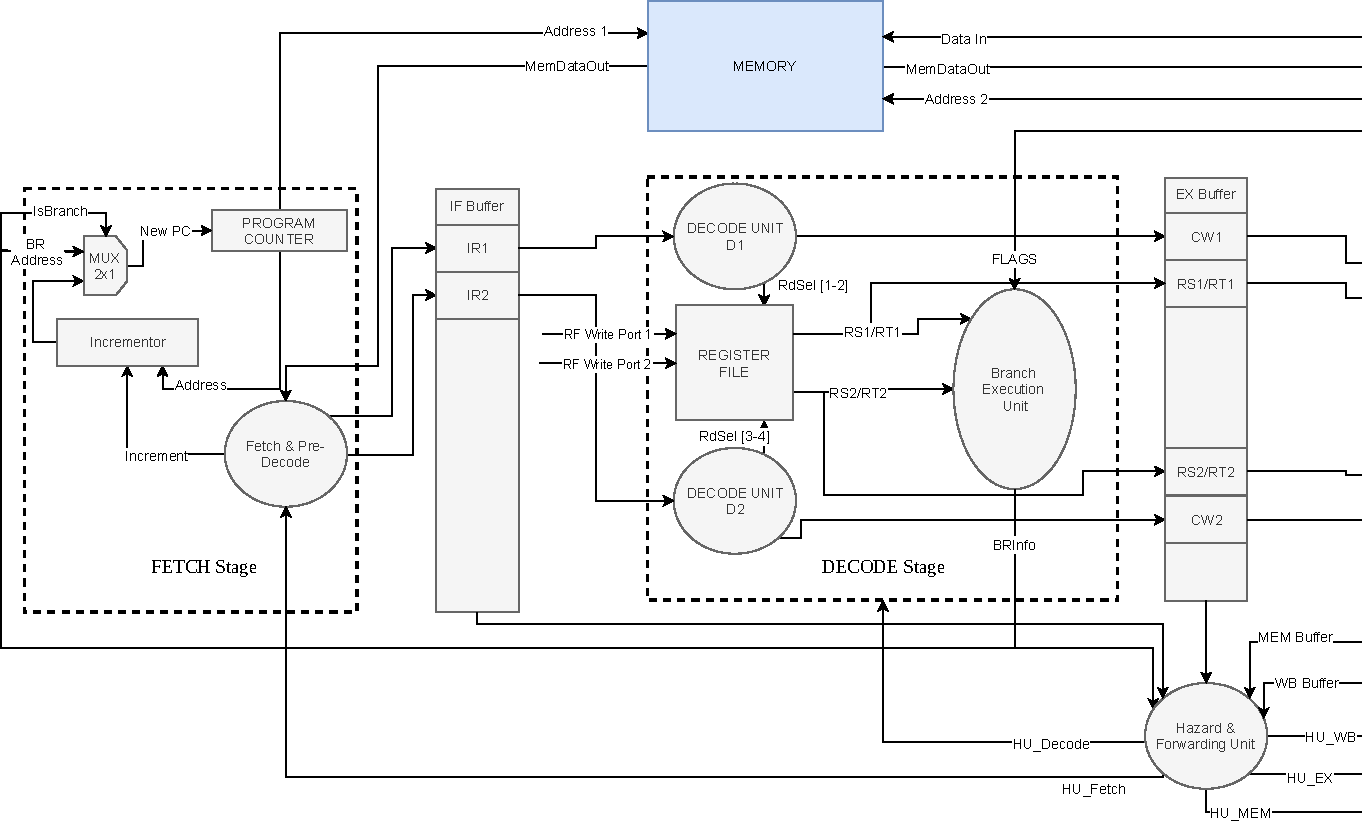
\includegraphics[page=1]{Diagrams/SystemOverviewSplit}
        \caption{Overall Schematic Part 1}
        \label{sys-schematic-1}
    \end{sidewaysfigure}
    \begin{sidewaysfigure}[h]b
        \centering
        \includegraphics[page=2]{Diagrams/SystemOverviewSplit}
        \caption{Overall Schematic Part 2}
        \label{sys-schematic-2}
    \end{sidewaysfigure}

\subsection{Memory Unit}
% TO-DO: DISCUSS THIS.
The memory block used is interfaced by two address lines, with the second line given priority whenever a read / write is requested by it. A single word is read or written when an address is on Address2. When an address is on the first line, \textbf{two words} are read at a time starting from the word at the address given by Address1. The first line is only for reading from the memory and has no write option. The read operation is instantaneous while the write operation takes 1 clock cycle (the value is written onto the memory on the falling edge of the clock). 

\subsection{Fetch Stage}
In the fetch stage, the Program Counter (PC) register is connected to Address1 of the memory, the data is then read into the fetch and pre-decode unit which has three outputs: the IRs (Instruction Registers) corresponding to the two streams in Orthrus, IR1 and IR2, as well as the increment to add to the PC for fetching the next instruction. The key point is that the pre-decode unit must do not let two memory-accessing instructions simultaneously into the two streams (since this would result in a structural hazard) and hence passes a No-Op into the second stream when this is detected. The pre-decode unit also passes a No-Op into the second stream when an immediate instruction is loaded, since an immediate instruction takes two words. The pre-decode unit must also pass a No-Op when the two instructions try to use the output port. To reduce hardware complexity, a CALL must always be in the first stream, and a No-Op is inserted to fix that if it is not the case. The flow chart for the unit's operation is given by Figure~\ref{fetch-pre-decode-unit}. For the flow chart, the instructions that access memory are: PUSH / POP / LDD / STD / CALL / RET / RTI. In addition to the pre-decoding unit mentioned, the fetch stage also includes an incrementor to increment the PC as well as a small unit (shown in Figure~\ref{fetch-predecode-npc}) to choose whether to get the PC from the incremented PC, normal branches, or from RET / RTI / ITR (which are executed in the last stage by necessity of fetching from memory).

\begin{figure}
    \centering
    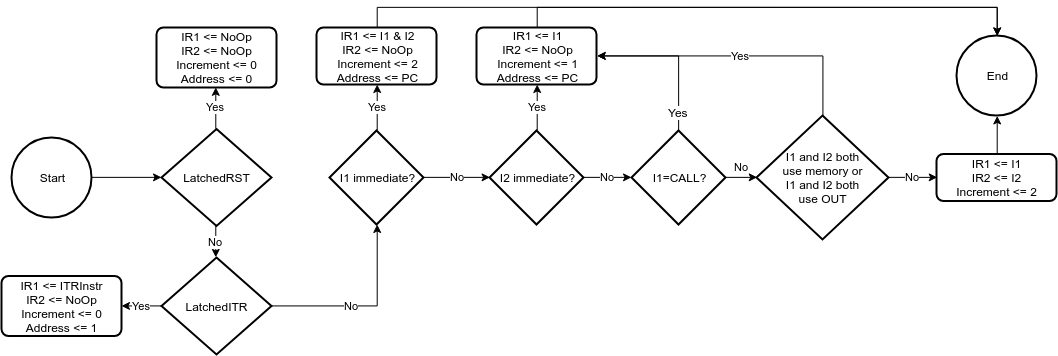
\includegraphics[width=\textwidth]{Diagrams/fetch_predecode_su}
    \caption{Fetch and Pre-Decode Unit Operation}
    \label{fetch-pre-decode-unit}
\end{figure}

\begin{figure}
    \centering
    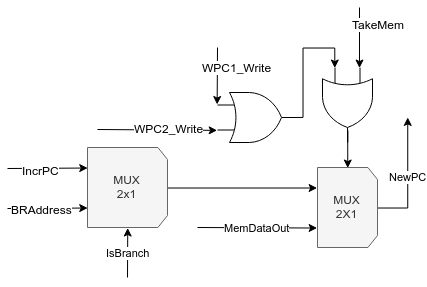
\includegraphics{Diagrams/fetch_predecode_npc.png}
    \caption{Next PC MUXing Unit}
    \label{fetch-predecode-npc}
\end{figure}

\subsection{Decode Stage}

\subsection{Execute Stage}

\subsection{Memory Stage}

\subsection{Write Back Stage}

\subsection{Hazard Detection Unit}

\subsection{Branching}


% --------------------------------------------------------------
%     You don't have to mess with anything below this line.
% --------------------------------------------------------------
			
\end{document}	